\section{Branches} \label{section: branches}

\subsection{Definitions}

Our team will use a sprint methodology.
Sprints will last four weeks, and short-lived branches will exist for no more than one sprint.
Long-lived branches will exist indefinitely.
During each sprint, many features will be implemented, culminating in a release at the end of the sprint.
One integrator will direct the sprint, serving multiple roles (approving pull requests, assigning tasks, leading the resolution of merge conflicts, etcetera).
The integrator’s roles will be covered below.

The branch structure is shown in \Cref{fig:git-workflow}.

 \subsection{Long-Lived Branches}

 Three long-lived branches will persist between sprints. Their purposes are as follows:

 \begin{itemize}
    \item \textbf{Main}:
    The Main branch tracks major versions (1.0, 2.0, 3.0…) and will typically be updated once for each deliverable, once all tasks for that deliverable are completed. The release branch will be merged to Main once per sprint at most, but Main will not necessarily be updated every sprint. Code will only be merged directly to Main in the case of emergency hotfixes which have no structural impact. Feature development never occurs in Main. Only the integrator has permission to merge the Release branch into main or hotfix Main. No one else on the team is permitted to update Main. No branch pulls from Main.
    \item \textbf{Release}:
    The Release branch tracks minor versions (1.1, 1.2, 1.3…) and is updated once per sprint, at the end of every sprint. It collects all features completed during that sprint. At the end of the sprint, the Develop branch is merged into Release and given a version number. Code will only be merged directly to Release in the case of emergency hotfixes which have no structural impact. Feature development never occurs in Release. Only the integrator has permission to merge into release or make hotfixes. Release never pulls from Main – Instead, updates are pushed from the Develop branch to Release, and then to Main.

    \item \textbf{Develop}:
    The Develop branch does not have version numbers, as it is continuously changing during a sprint. As developers complete features, they send pull requests to the integrator. By the time a pull request has been sent to Develop, the feature has already been thoroughly tested. If a merge conflict occurs due to a pull request, the integrator is responsible for examining the conflict and resolving it. If the conflict is especially difficult and complicated, the integrator may have the feature developer assist in resolving it. Develop never pulls from Release or Main, it exists in a one-way relationship. Code is never added directly to Develop – instead, feature branches are created with the change, and a pull request is made. The integrator is the only team member with permission to merge features into Develop, or to hotfix Develop when necessary.
 \end{itemize}

 \subsection{Short-Lived Branches}

 All members of the team, other than the integrator, do all their work in short-lived branches.
 The only permission they have is to create short-lived branches and pull requests.
 These short-lived branches are deleted upon being merged and should live for no longer than one sprint.
 Each short-lived branch should track exactly one issue.

 \begin{itemize}
    \item \textbf{Feature Branches}: Feature branches are where most active development occurs. Team members will create a new branch from Develop and implement their desired changes. Each feature branch contains an issue number in its name for purposes of linking, and each feature branch targets exactly one issue. Team members may frequently pull from Develop to feature branches during work on a feature to avoid merge conflicts. As soon as features are successfully merged to Develop, the branch is deleted.
    \item  \textbf{Hotfix Branches}: Sometimes, a hotfix is necessary, but it may be very complex or require the expertise of a team member other than the integrator. In this case, it is useful to create a Hotfix branch rather than directly hotfix the target branch. This is especially important when a non-integrator will assist with a hotfix, because they do not have permission to commit to long-lived branches. These hotfix branches are still manually approved by the integrator and held to the same testing standard as any other branch. Hotfixes, whether from a branch or directly implemented, are tagged with a third version number such as 1.0.1, 1.0.2, 1.0.3, etc. 
 \end{itemize}

 \begin{figure*}
\centering
    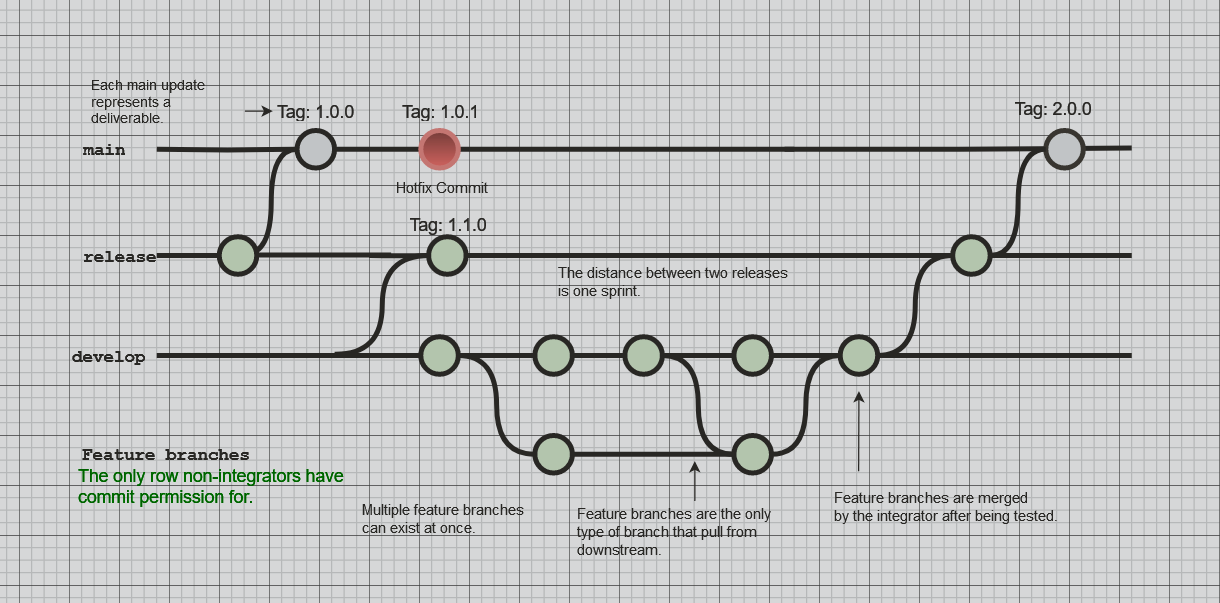
\includegraphics[width=0.9\linewidth]{Figures/git-workflow.png}
    \caption{Git Workflow Representation}
    \label{fig:git-workflow}
    %\vspace{-5mm}
\end{figure*}

